\chapter{Conclusions and Future Work}
\label{conclusions_and_future_work}

\section{Summary and Conclusions}

In this upgrade thesis, I have detailed the work I have done so far in my PhD: explored survival analysis in MND, developed a Python library called Fusilli for the machine learning methods I will apply to multimodal MND data, and applied Fusilli to MND data for prognosis prediction.

\subsection{Cox model}

Chapter~\ref{cox_proportional_hazards_model} showed the application of a Cox proportional hazards model to multimodal MND data, comprised of baseline clinical features and brain region volumes extracted from structural MRI near diagnosis.
To my knowledge, combining clinical and MRI-derived features in survival analysis for MND has only been done in one other paper~\cite{querinSpinalCordMultiparametric2017}, which used spinal cord MRI data and a smaller sample size.
The main contribution of this chapter was to show that the Cox model could be used to predict prognosis in MND, and that the resulting factors significantly affecting survival are changed when using clinical data, imaging data, or multimodal data.

The main result was that when using clinical data and extracted brain region volumes from MRI, the most important factors affecting survival were the baseline ALSFRS-R score and the bilateral volume of the amygdala, which were protective of survival, and the ALS-subtype of MND and larger bilateral lateral ventricle volumes, which were detrimental to survival.
The addition of MRI data to clinical information caused a change in the relevance of specific clinical variables within the model, which implied that the brain volumes derived from MRI scans included corresponding information to some clinical features.
In contrast, depending simply on MRI data produced clinically unusual outcomes.
The implications of these findings highlighted the importance of combining imaging data with clinical information for more meaningful survival analysis in MND.


\subsection{Fusilli}

In Chapter~\ref{fusilli_development}, I showcased Fusilli, my Python library for easy comparison of multimodal data fusion methods, and the steps in its development.
Fusilli is an open-source project, and therefore released for anybody to use in their personal projects.

Key contributions of this chapter were the development of a library that has a catalogue of multimodal data fusion methods that are not limited by their underlying architecture, which is the general limitation of other similar works.
Fusilli was received with interest by the machine learning community, and I have received feedback from other researchers who have used Fusilli in their own projects.

For my future PhD chapters, using Fusilli will greatly speed up my analysis and experimentation.

\subsection{Fusilli with MND data}

My first experimentation with Fusilli for MND prognosis prediction is shown in Chapter~\ref{fusilli_on_mnd}.
The experiment consisted of using baseline clinical data and extracted brain region volumes to predict whether a patient with survive for more or less than 24 months from diagnosis.
Eight multimodal data fusion models, implemented in Fusilli, were compared to each other and to unimodal models.

This experiment resulted in only one of the multimodal models outperforming the unimodal model that used only clinical data, when evalutaing with balanced accuracy.
Inspection of the validation performance revealed that the models were overfitting to different degrees, and further hyperparameter tuning is needed to improve the models to be more generalisable.

The implications of this were that, in its current form with a small sample size and limited hyperparameter tuning, Fusilli did not show a clear advantage of using multimodal data in MND prognosis prediction, and that imaging data may not have been as useful as clinical data in this task.

Further investigation and experimentation is needed to determine the finality of these results.
I hypothesise that with more data, better clinical characterisation, and more fine-grained imaging data, multimodal data fusion will prove to be a useful tool in MND prognosis prediction.

\section{Future Work}

I have split the possible future work sections into roughly three chapters.
Most of the work described here relies on the availability of a larger sample size of data from MND cohorts.
Currently, my supervisory team and I are liaising with other researchers for access to more data, as well as applying for access to MRI scans from UCLH (University College London Hospitals), which correspond to subjects in ALS Biomarkers Study.

Moreover, I am undertaking a research visit to Charité - Universitätsmedizin Berlin in April and May of 2024, where I will be working on extending Fusilli's capabilities and applying Fusilli to multimodal medical data on mental health and addiction disorders.
I will be making connections and collaborating with researchers at Charité, and while I am there, I hope to visit MND clinics in Berlin to improve my understanding of other areas of MND clinical research.

\subsection{Applying Fusilli to multimodal medical data: MND and other applications}

The next step in my PhD is to continue to apply Fusilli to MND data, especially with larger sample sizes and more tuning of hyperparameters.
I will also apply Fusilli to other multimodal medical datasets to round out the development of the library, by showing what Fusilli can do in multiple applications.

\subsubsection*{Illustrating Fusilli capabilities with multimodal medical data}

Although Chapter~\ref{fusilli_development} showed the whole development journey of Fusilli, a valuable addition to the narrative would be to show how Fusilli can be used in practice.
My plan is to use Fusilli ``out-of-the-box" on two multimodal medical datasets: one on neurodegenerative diseases and one on critical care chest X-rays.

In terms of feasibility, I already have access to ADNI (Alzheimer's Disease Neuroimaging Initiative) and PPMI (Parkinson's Progression Markers Initiative) data for neurodegenerative diseases, and MIMIC CXR (Medical Information Mart for Intensive Care - Chest X-ray) data for critical care.

To finish this analysis off, I will first need to download the data, for which I will ask for assistance from colleagues at Centre for Medical Image Computing (CMIC) who have used these datasets before.
Secondly, I will need to preprocess the data by dealing with data missingness in clinical data and running preprocessing pipelines on the imaging data: segmentation and registration for MRI data, and preprocessing for chest X-ray data.
Next, I will choose a task to apply Fusilli to, such as prognosis prediction or disease classification, and I will seek clinical advice on the most appropriate task for each dataset.
Finally, I will run the Fusilli pipeline on the data, and analyse the results.

\subsubsection*{Extending work on applying Fusilli to MND prognosis prediction}

In Chapter~\ref{fusilli_on_mnd}, I showed the first application of Fusilli to MND data.
The next step is to extend this work by using more data from collaborations and the ALS Biomarkers Study, and by fine-tuning the parameters and architectures of the fusion models, in order to increase the accuracy of the predictions and more definitively assess the utility of multimodal data in MND prognosis prediction.
I plan to do this work alongside applying Fusilli to non-MND data, as described above.

The first step in improving the models would be to examine our preprocessing and feature inclusion of clinical data.
The main additional clinical feature to be added to the analysis would be neurofilament light chain (NfL) measurements from the ALS Biomarkers Study, which are currently too sparse to be used in the models so far, but samples are being analysed to increase the number of measurements available.

Furthermore, collaborators in Jena are running their D50 model on the ALS Biomarkers Study ALSFRS-R data.
Using the D50 will enable the estimation of the ALSFRS-R at the date the MRI was taken, which will allow us to use MRI data from further away from diagnosis alongside the clinical data.
It will also allow us to investigate the effect on performance when preprocessing the ALSFRS-R data in different ways, such as using the raw scores, the slopes of the raw scores, which have shown promise in a recent paper~\cite{papaizEnsembleimbalancebasedClassificationAmyotrophic2024}, or the D50-estimated ALSFRS-R.
Moreover, we will obtain D50-derived parameters of disease aggressiveness and accumulation, which could be used as added features in the models.

For the imaging data, we will obtain more fine-grained brain measurements from using the \texttt{recon-all} pipeline from FreeSurfer, and use feature selection methods and domain knowledge to decide which measurements to include in the models.

The expected outcomes of this work are more accurate predictions of MND prognosis, and a better understanding of the utility of multimodal data in MND prognosis prediction.

\subsection{Effect of MRI preprocessing on Fusilli prognosis prediction}

% to write

Moving onto applying multimodal methods to actual images with clinical data.

Looking at the effect of various image preprocessings.
We showed that there is not consensus on the areas of the brain that are most important in MND, so we could look at the effect of different preprocessing pipelines on the performance of the models.

Examples are focusing on cortical thickness, subcortical volumes, whole brain measurements, and also other preprocessing steps such as texture analysis.

Deji is working on upscaling the clinical-grade scans to research-grade scans, which will allow us to use the scans in the models as whole-brain images and more easily apply these preprocessing steps.

Some toolkits I am planning on using are: the texture analysis one from canada, recon-all, ...
- texture analysis: https://github.com/ajinkya-kulkarni/PyTextureAnalysis?tab=readme-ov-file
- recon-all


The quality of the inferences taken from this analysis will depend on the sample size of the data, because imaging is more expensive to process than clinical data, and a larger sample size would mitigate the less useful result of ``less features leads to less overfitting".

If the sample size is not large enough, a contigency plan would be to focus on diseases that have more data available, such as Alzheimer's disease.

\subsection{Final project options}

% to write

The final project in this PhD will depend on the availability of data.
We could either add more data modalities to the multimodal models, such as spinal MRI or features derived from radiological reports, or we could investigate the usefulness and sensitivity of the best-performing models on varying definitions of prognosis.

\subsubsection*{Sensitive analysis of Fusilli prognosis prediction on varying prognosis definitions}

Looking at different prognosis outcomes, such as survival, ALSFRS-R decline, or other measures of disease progression, could provide a more nuanced understanding of the performance of Fusilli.

\subsubsection*{Adding spinal cord MRI data to Fusilli prognosis prediction}
Dependent on data availability
\begin{itemize}
    \item Motivation: spinal cord is important in MND, example papers to show this
    \item Feasibility: Access to spinal cord MRI data
\end{itemize}

\subsubsection{Adding radiological report derived features to Fusilli prognosis prediction}
Dependent on data availability
\section{Timeline}

\begin{figure}
    \centering
    \hspace*{-0.1\textwidth}
    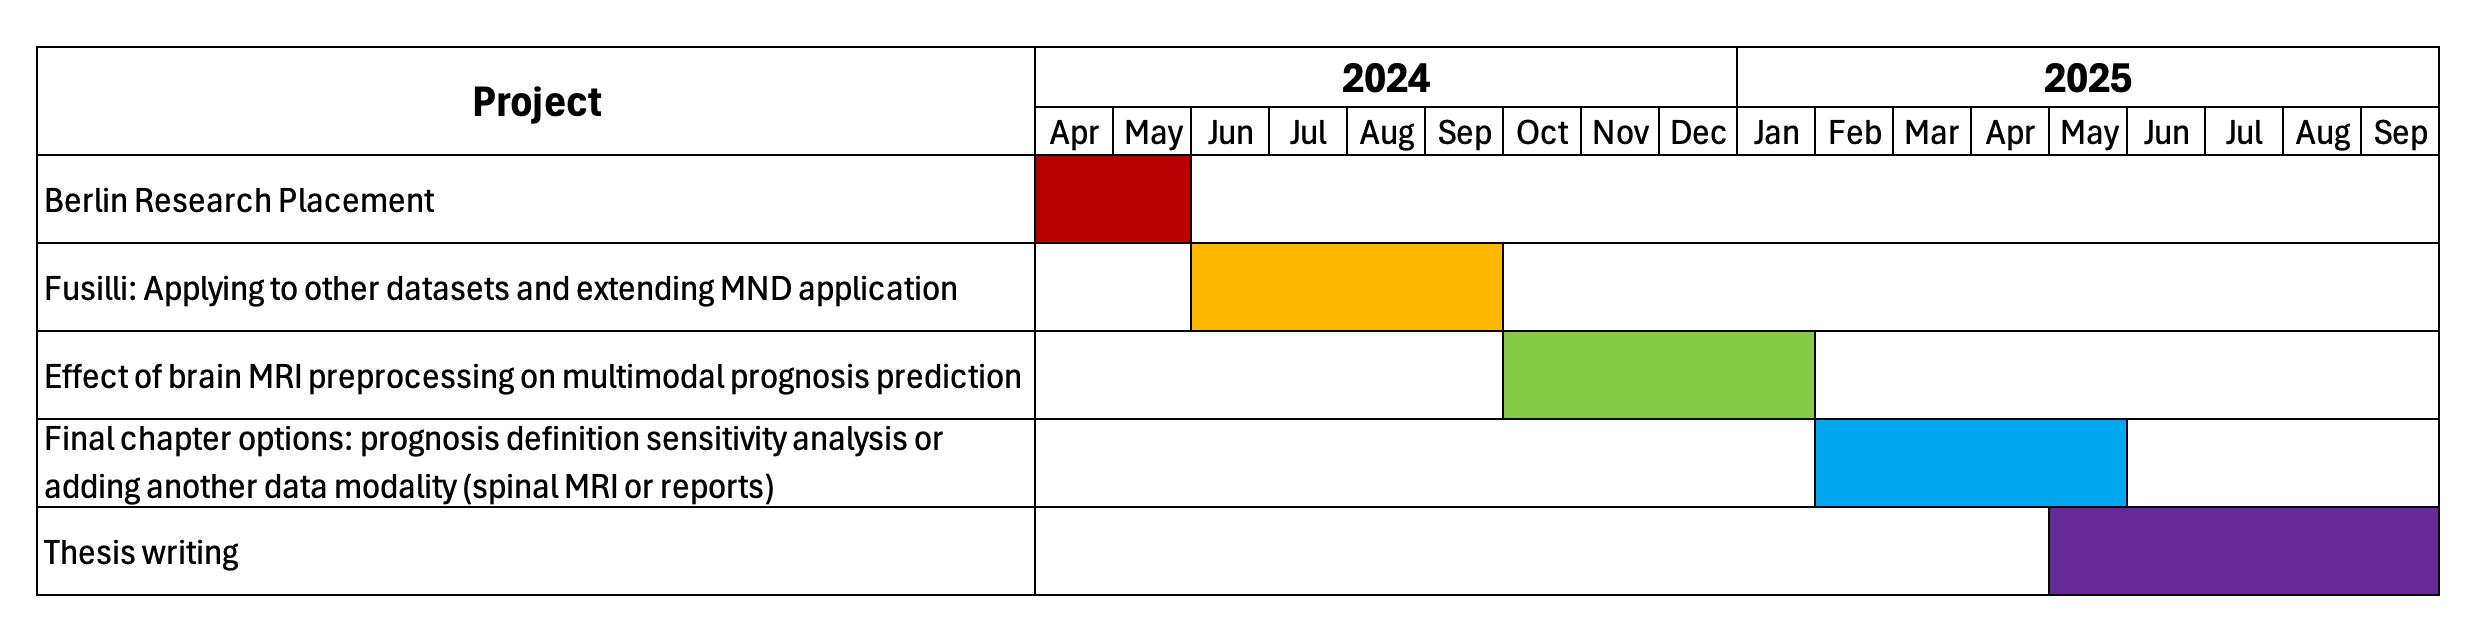
\includegraphics[width=1.2\textwidth]{figures/gantt_chart}
    \caption{Gantt chart showing the timeline for the remaining work in my PhD}
    \label{fig:gantt_chart}
\end{figure}

\begin{itemize}
    \item What have I done so far? Papers and conference submissions
    \item Outcomes for the rest of my PhD
    \begin{itemize}
        \item Papers
    \end{itemize}
    \item Gantt chart
\end{itemize}
